\documentclass[12pt,oneside]{amsart}
\usepackage{amsmath}
\usepackage{lipsum}
\usepackage{multicol}
\usepackage{caption}

\linespread{1.5}

% Adjust page margins and spacing
\setlength{\topmargin}{-0.5in}       % reduce top margin
\setlength{\textheight}{9.5in}       % increase usable vertical space
\setlength{\oddsidemargin}{-0.1in}    % reduce side margins
\setlength{\evensidemargin}{-0.1in}   % ensure consistency
\setlength{\textwidth}{6.7in}        % increase usable horizontal space

% Caption settings
\usepackage[font=small,labelfont=bf]{caption}
\captionsetup{width=\linewidth, font=scriptsize, skip=2pt}
\captionsetup[figure]{belowskip=-10pt}
%-------Packages---------
\usepackage{amssymb,amsfonts}
\usepackage[all,arc]{xy}
\usepackage{enumerate}
\usepackage{mathrsfs}
\usepackage{graphicx}
\usepackage{epstopdf}
\usepackage{listings}
\usepackage{appendix}
\usepackage{listings}
\usepackage{placeins}
\usepackage{booktabs}
\usepackage{tabularx}
\usepackage{float}
\usepackage{hyperref}
\usepackage[hypcap=true]{caption}


%--------Theorem Environments--------
%theoremstyle{plain} --- default
\newtheorem{thm}{Theorem}[section]
\newtheorem{cor}[thm]{Corollary}
\newtheorem{prop}[thm]{Proposition}
\newtheorem{lem}[thm]{Lemma}
\newtheorem{conj}[thm]{Conjecture}
\newtheorem{quest}[thm]{Question}

\theoremstyle{definition}
\newtheorem{defn}[thm]{Definition}
\newtheorem{defns}[thm]{Definitions}
\newtheorem{con}[thm]{Construction}
\newtheorem{exmp}[thm]{Example}
\newtheorem{exmps}[thm]{Examples}
\newtheorem{notn}[thm]{Notation}
\newtheorem{notns}[thm]{Notations}
\newtheorem{addm}[thm]{Addendum}
\newtheorem{exer}[thm]{Exercise}

\theoremstyle{remark}
\newtheorem{rem}[thm]{Remark}
\newtheorem{rems}[thm]{Remarks}
\newtheorem{warn}[thm]{Warning}
\newtheorem{sch}[thm]{Scholium}
\newcommand{\be}{\begin{equation}}
\newcommand{\ee}{\end{equation}}
\makeatletter
\let\c@equation\c@thm
\makeatother
\numberwithin{equation}{section}

\usepackage[style=apa,sortcites=true,sorting=nyt,backend=biber,natbib=true]{biblatex}
%bibliographystyle{unsrtnat}
\addbibresource{Reference/reference.bib}
%%%%%%%%%%%%%%%%%%%%%%%%%%%%%%%%%%%%%%%%%%%%%%%%%%%%%%%%%%%%%%%%%%%%%%%%%%%%%%%%%
% your title/author/date information go here
%--------Meta Data: Fill in your info------


\title{On the Multiple Imputation}

\author{Xuan Li}

\date{April 8, 2025}

\begin{document}

\begin{abstract}
    This report serves as a qualifying paper for the UBC Statistics PhD program, providing a summary of the paper “Multiple Imputation: A Review of Practical and Theoretical Findings” \citep{qp}. The paper offers a broad overview of multiple imputation (MI), covering both theoretical foundations and practical considerations. In this report, we briefly highlight some key theoretical results and practical insights discussed in the review paper. Building on this foundation, we conduct an extensional study that focuses on evaluating the performance of parametric versus nonparametric imputation methods for a single continuous variable under varying data-generating processes and levels of missingness. Our results suggest that parametric methods perform well when their assumptions align with the underlying data structure but degrade under model misspecification, while nonparametric methods offer greater robustness at the cost of increased uncertainty. Our findings also underscore the importance of considering data complexity and missingness mechanisms when selecting imputation strategies.
\end{abstract}
\maketitle
\tableofcontents

%%%%%%%%%%%%%%%%%%%%%%%%%%%%%%%%%%%%%%%%%%%%%%%%%%%%%%%%%%%%%%%%%%%%%%%%%%%%%%%%%section 1


\section{Introduction}
Missing data is a common issue in applied statistical analysis, and improper handling can lead to biased estimates and invalid inferences. Multiple Imputation (MI), originally developed by Rubin \citep{rubin}, offers a principled framework to address this challenge. Instead of filling in missing values with single estimates, MI generates multiple plausible versions of the incomplete dataset. Each completed dataset is analyzed separately, and the results are combined to incorporate both within-imputation and between-imputation uncertainty. MI is particularly appealing because it provides valid statistical inference under relatively mild assumptions, most notably when data are missing at random (MAR). However, its effectiveness hinges critically on the compatibility between the imputation model and the underlying data structure, as well as the validity of assumptions about the missingness mechanism.

This report aims to both summarize and extend some key insights from the paper "Multiple Imputation: A Review of Practical and Theoretical Findings" \citep{qp}. The paper provides a comprehensive overview of the statistical foundations and practical considerations underlying MI. In this report, we firstly go through several central concepts discussed in the review. Building on this foundation, we then conduct our extensional study. Given the breadth of topics discussed in the original review paper, the extensional study focuses on a single but important direction: evaluating the performance of parametric versus nonparametric imputation methods for a single continuous variable under varying data-generating processes and missing data proportion. This choice reflects the emphasis on model compatibility and misspecification as critical concerns in practice. This extension aims to provide practical insights into the sensitivity of multiple imputation when model assumptions are violated or approximately satisfied.

\section{Summary of the Review Paper}
The original review paper is broad in scope, offering both theoretical depth and practical guidance across a wide range of imputation methods. It begins with foundational settings involving a single variable with missing values, and then extends to more complex cases where multiple variables are subject to missingness. 

In these multivariate contexts, the paper explores three different imputation frameworks. The first is \textbf{Joint Modeling (JM)}, particularly the \textbf{simultaneous} approach, which specifies a full multivariate distribution for all variables, typically assuming multivariate normality. The second is \textbf{Fully Conditional Specification (FCS)}, or chained equations, which models each variable conditionally on all others. Lastly, the paper introduces a \textbf{Sequential Joint Modeling} approach, which builds the joint distribution as a product of univariate models ordered in sequence. These methods are analyzed in terms of their theoretical guarantees, flexibility, and practical trade-offs. 

The review also covers the concept of \textbf{congeniality} and \textbf{proper imputation}, explaining their importance for valid inference in MI. It also discusses when imputations can be considered \textbf{valid} under both Bayesian and frequentist perspectives. 

Additionally, it mentions some existing imputation model diagnostics and highlights the growing use of nonparametric and machine learning methods. By synthesizing theoretical results with practical insights, the review serves as a valuable and comprehensive resource for practitioners and researchers.

\subsection{Key Theoretical Results}
We begin with introducing the following notations and definitions as in the review paper. Let $Y_i = (Y_{i1}, \ldots, Y_{ip})$ be a $p$-dimensional vector for observation $i$, we denote 
\begin{itemize}
    \item $M$ as the total number of imputed datasets,
    \item $Y_{\text{obs}}$ as the observed portion of the dataset, and $Y_{\text{mis}}^{(m)}$ as the $m$-th imputation of the missing data,
    \item $Q$ as the the \textbf{parameter of interest} (e.g., a mean, a regression coefficient),
    \item $\hat{Q}^{(m)}$ be the estimator computed from the $m$-th completed (imputed) dataset.
\end{itemize}
Under the assumption that the missing data mechanism is \textbf{Missing at Random (MAR)}, MI generates multiple completed datasets from the posterior predictive distribution of $Y_{\text{mis}}$ given $Y_{\text{obs}}$. Each completed dataset after imputation is then analyzed using the estimator $\hat{Q}^{(m)}$, and the results are pooled using Rubin’s combining rules.

From \citep{rubin}, the following quantities are defined:
\begin{enumerate}
    \item \textbf{Mean of the MI Estimators:}
    \[
    \bar{Q}_M = \frac{1}{M} \sum_{m=1}^{M} \hat{Q}^{(m)}
    \]
    
    \item \textbf{Within-Imputation Variance:}
    \[
    \bar{U}_M = \frac{1}{M} \sum_{m=1}^{M} \hat{U}^{(m)}
    \]
    where $\hat{U}^{(m)}$ is the variance of $\hat{Q}^{(m)}$ within each imputed dataset.
    
    \item \textbf{Between-Imputation Variance:}
    \[
    B_M = \frac{1}{M - 1} \sum_{m=1}^{M} (\hat{Q}^{(m)} - \bar{Q}_M)^2
    \]
    which captures variation in $\hat{Q}^{(m)}$ across different imputations, reflecting uncertainty due to missing data.
\end{enumerate} 
The \textbf{total variance} in MI is given by:
\begin{equation}
    T_M = \bar{U}_M + \left( 1 + \frac{1}{M} \right) B_M.
\end{equation}
The total variance $T_M$ captures both the within-imputation uncertainty and the additional variability introduced by the imputation process itself.

\textbf{Why and When Does MI Work?}  
The review provides a theoretical foundation for the validity of MI from both Bayesian and frequentist perspectives. Under the Bayesian framework, multiple imputation delivers valid inference if the imputer and analyst share the same distribution:
$$
P_I(Y_{\text{mis}} \mid Y_{\text{obs}}) = P_A(Y_{\text{mis}} \mid Y_{\text{obs}}),
$$
then, each imputed estimate $\hat{Q}^{(m)}$ can be viewed as a draw from the analyst’s posterior distribution for $Q$: $$
P_A(Q \mid Y_{\text{obs}}) = \int P_A(Q \mid Y_{\text{mis}}, Y_{\text{obs}}) P_A(Y_{\text{mis}} \mid Y_{\text{obs}}) \, dY_{\text{mis}}. 
$$
If the posterior is approximately normal and the number of imputations $M$ is not too small, then the MI statistics—$\bar{Q}_M$, $\bar{U}_M$, $B_M$, $T_M$—provide a reasonable approximation to the posterior mean and variance.  

However, in practice, Bayesian validity is rarely attained. The imputer and the analyst often use different models or priors, leading to a mismatch between $P_I(Y_{\text{mis}} \mid Y_{\text{obs}})$ and $P_A(Y_{\text{mis}} \mid Y_{\text{obs}})$. As a result, MI is typically evaluated based on its \textit{frequentist} properties—specifically, its behavior under repeated sampling. From a frequentist perspective, the validity is justified under two main assumptions:
\begin{itemize}
    \item \textbf{Assumption 1: Confidence Validity of Complete-Data Inference.} The complete-data estimator $\hat{Q}(Y)$ must yield confidence intervals with at least nominal coverage. This requires the estimator to be approximately unbiased, and its variance estimate $\hat{U}$ to not underestimate the true sampling variability.
    \item \textbf{Assumption 2: Asymptotic Normality of the Sampling Distribution.} The sampling distribution of $\hat{Q}$ is assumed to be approximately normal, so that confidence intervals can be validly constructed using $\hat{Q}$ and $\hat{U}$.
\end{itemize}
When these conditions hold, multiple imputation (MI) provides valid frequentist inference. In practice, these assumptions may only hold approximately—especially in small samples or complex models.


\textbf{Proper Imputation and Congeniality.} 
To ensure frequentist validity in finite samples, Rubin introduced the concept of \textbf{proper} imputation \citep{rubin}, which refers to an imputation procedure that, when combined with valid complete-data inference, yields valid MI inference. Proper imputation ensures valid inference for a specific estimand and missingness mechanism by accounting for both the uncertainty due to missing data and the variation from sampling. \textbf{Congeniality}, a concept introduced by Meng \citep{meng}, addresses Bayesian validity and requires the alignment between the imputer’s and analyst’s models. While proper imputation can yield valid inference even in the presence of uncongeniality especially when the imputation model is more saturated, confidence validity is not guaranteed if the mismatch between models is too severe. In short, valid inference under MI requires proper imputation, benefits from congeniality, but can often withstand mild uncongeniality when applied thoughtfully.

\subsection{Practical Findings}
While the theoretical foundations of multiple imputation (MI) are well-established, its effective use in practice hinges on several key modeling choices. The review paper highlights three major practical recommendations: reflecting uncertainty, including sufficient variables, and using flexible imputation models.

\textbf{1. Reflecting Uncertainty.}
 A core requirement for valid inference under MI is that the imputation process must reflect not only the uncertainty about the missing values but also about the imputation model itself. This means incorporating stochastic variation in the imputation step—such as through Bayesian draws or bootstrapping techniques—rather than relying on deterministic estimates.

\textbf{2. Include Sufficient Covariates.}
 The review paper mentions that imputation models should, whenever possible, include all relevant variables—especially those that may be used in downstream analyses. Omitting important covariates can result in improper imputations and bias in the final estimates, particularly when the imputer and analyst are not the same. In contrast, including additional (even irrelevant) covariates may increase variance slightly but does not introduce bias. 

\textbf{3. Favor Flexible Models.}
 According to the paper, flexible imputation models—such as nonparametric or semiparametric approaches—are more capable of adapting to complex data structures. These models are especially valuable when the imputer has limited knowledge about the correct functional form or lacks time to iteratively refine models. While incorporating prior information and controlling for model fit in flexible frameworks can be more challenging, both theoretical and empirical findings suggest that simple imputation models—such as multivariate normal models or PMM with only linear main effects—should be used with caution and carefully scrutinized.
 
Overall, these considerations emphasize a shift toward richer, more adaptive imputation procedures. As MI is increasingly applied in complex real-world scenarios, the importance of these modeling choices cannot be overstated. In multivariate settings, While JM methods provide a coherent probabilistic framework, FCS methods offer greater flexibility, especially for mixed data types. However, the practical considerations discussed above—propagating uncertainty, including sufficient covariates, and using flexible models—remain equally critical regardless of the imputation framework used.


\subsection{Limitations and Future Works}
While the review paper offers a broad and insightful overview of multiple imputation (MI) methods—covering theoretical foundations, practical recommendations, and comparisons between approaches—there are also limitations for further investigation.

\begin{itemize}
    \item Many of the theoretical results regarding consistency, efficiency, and validity of MI methods assume either correctly specified models or rely heavily on parametric assumptions. However, the paper does not go into a depth analysis of how well different imputation strategies (such as parametric and nonparametric methods) handle model misspecification. 
    \item The analysis in the review paper relies on the setting of the MAR missing mechanism. In practice, verifying MAR is difficult, and real-world data often violate this assumption. This limits the applicability of the theoretical guarantees presented. Future extensions could explore how MI performs under violations of MAR, such as Missing Not At Random (MNAR) scenarios, or develop diagnostic tools to assess the plausibility of the MAR assumption in applied settings.
    \item The paper introduces the theoretical concept of congeniality but provides little insight into how practitioners can detect or diagnose uncongeniality or model misspecification in real applications.
    \item While the review advocates for including all relevant variables in the imputation model, it offers limited practical guidance on how to select "relevant" variables in different analytic contexts. The trade-off between improving prediction and risking overfitting or uncongeniality is not fully explored.
    \item While the paper encourages using multiple imputation for a wide range of estimands, much of the theoretical development and empirical illustration centers on the common ones like mean estimation. More work is needed to evaluate MI involving complex estimands and small sample conditions. The precision of variance estimates under these conditions is especially critical.
    \item The review lacks concrete recommendations on how to choose imputation models tailored to specific data types, such as categorical, ordinal, mixed, or longitudinal data structures. And the paper could have been strengthened by comparing how different MI methods perform across common statistical software packages, helping applied users understand the trade-offs involved in implementation choices.
    \item Finally, although the authors mention some directions for evaluation and suggest simulation as a practical approach to compare imputation methods, they do not provide standardized designs or benchmarks. There is a growing need to establish common evaluation frameworks that incorporate both theoretical alignment and practical performance under controlled but realistic conditions.
\end{itemize}

\section{Extensional Study}
The extensional study focuses on the case of a single continuous missing variable and evaluating MI performance under varying proportions of missing data. We firstly explore some theoretical analysis and then move forward with practical simulations. Specifically, we compare parametric and nonparametric imputation methods across two data-generating scenarios (linear and polynomial), assuming the primary estimand of interest is the sample mean. Future work could expand this design to explore additional estimands (e.g., quantiles, treatment effects), more complex missing data mechanisms (e.g., MNAR), and higher-dimensional data settings.

\subsection{Variance in MI relative to Missing Data Proportion}
To theoretically explore how missing proportion might affect variance in imputed datasets, we focus on a \textbf{simplified setting} where we are interested in estimating the \textbf{mean} of a \textbf{single continuous variable $y$}. In our case, we assume that only one variable $Y_i$ (scalar) contains missing values, and the other variable(s), if any, are fully observed and used as predictors during imputation. We further assume the following:
\begin{itemize}
    \item $Y_i$ are independently and identically distributed (i.i.d.) with finite variance $\sigma^2$,
    \item The missing data mechanism is \textbf{Missing Completely at Random (MCAR)}, so the observed data are a random subsample of the full data,
    \item The estimator of interest $Q$ is the sample mean $\hat{Q} = \frac{1}{n} \sum_{i=1}^n Y_i$.
\end{itemize}
Under these conditions, the sampling variance of the complete-data mean estimator (i.e. if we had all $n$ observations) is given by:
\[
\text{Var}(\hat{Q}_{\text{complete}}) = \frac{\sigma^2}{n},
\]
where $\sigma^2$ is the \textbf{true population variance} of the underlying population for $Y$.
When a fraction $p$ of data is missing, the number of observed data points is:
\[
n_{\text{obs}} = (1 - p)n.
\]
Thus, the variance of $\hat{Q}$, with only the observed data, is:
\[
\text{Var}(\hat{Q}_{\text{obs}}) = \frac{\sigma^2}{(1 - p)n},
\]
due to $Y_{obs}$ being also a sample drawn from the true population $Y$ under the assumption \textbf{missing completely at random (MCAR)}. 

We introduce the variable $r$ as the relative increase in variance due to missingness. It is meant to quantify how much extra variance is introduced due to missing data. The variance of the estimator in the complete-data case, $\text{Var}(\hat{Q}_{\text{complete}})$, represents the variance of the estimator if we had all the data. In contrast, $\text{Var}(\hat{Q}_{\text{obs}})$ is the variance of the estimator with only the observed data. The difference between these variances tells us how much \textbf{information loss} occurs when we move from a complete dataset to an incomplete one.
\[
    r = \frac{\text{Var}(\hat{Q}_{\text{obs}}) - \text{Var}(\hat{Q}_{\text{complete}})}{\text{Var}(\hat{Q}_{\text{complete}})}
\]
Rearrange:
\[
\text{Var}(\hat{Q}_{\text{obs}}) = (1 + r) \text{Var}(\hat{Q}_{\text{complete}}).
\]
By substitution, we have:
\[
    \frac{\sigma^2}{(1 - p)n} = (1 + r) \frac{\sigma^2}{n} \Longrightarrow \frac{\sigma^2}{1 - p} = (1 + r) \sigma^2.
\]
Solving for $r$, we have:
\begin{equation}
r = \frac{\sigma^2}{(1 - p)\sigma^2} - 1 = \frac{1}{(1 - p)} - 1.
\end{equation}
To express the relative increase in variance due to missing data $r$ in terms of $B_M$ and $\bar{U}_M$, we follow Rubin's definition \citep{rubin}:
\[
r = \frac{B_M + B_M/M}{\bar{U}_M}.
\]
By rearrange and factor out $B_M$:
\[
B_M + \frac{B_M}{M} = r \bar{U}_M \Longrightarrow B_M \left(1 + \frac{1}{M}\right) = r \bar{U}_M.
\]
Solving for $B_M$, 
\begin{equation}
    B_M = \frac{r \bar{U}_M}{1 + \frac{1}{M}}.
\end{equation}
We now substituting the expression for $B_M$ in (3.2) to the total variance formula (2.1):
\[
T_M = \bar{U}_M + \left(1 + \frac{1}{M}\right) \cdot \frac{r \bar{U}_M}{1 + \frac{1}{M}}.
\]
Canceling $(1 + 1/M)$:
\[
T_M = \bar{U}_M + r \bar{U}_M = \bar{U}_M (1 + r).
\]
Thus, the total variance formula can be rewritten as:
\begin{equation}
    T_M = \bar{U}_M (1 + r).
\end{equation}
By substituting $r$ from earlier derivation (3.1) to the new formula for total variance (3.3), we have:
\[
T_M = \bar{U}_M \left(1 + \frac{1}{(1 - p)} - 1 \right).
\]
Simplify:
\begin{equation}
    T_M = \bar{U}_M \frac{1}{(1 - p)}.
\end{equation}
From (3.4), we observe several key interpretations:
\begin{itemize}
    \item If $p = 0$ (no missing data), then $T_M = \bar{U}_M$, which correspond to $B_M$ being zero. This is reasonable since in this case we observe no between-imputation variance. 
    \item If $p \to 1$ (almost all data missing), then $T_M \to \infty$, meaning inference becomes \textbf{unreliable}.
\end{itemize}
Although our exploration assumes $Q$ as the \textbf{mean estimator}, similar logic can be applied to other cases, provided that the variances are correctly specified for the given estimator. It is important to note that this is \textbf{not a formal proof, but a heuristic exploration} on the relationship between the missing proportion of data and the total variance under multiple imputation. Furthermore, many of the assumptions made here (such as MCAR, i.i.d. data) may not hold in real-world applications. In practice, the imputation model, estimator complexity, data structure, and missing data mechanism all interact to determine the actual variance properties after imputation.



\subsection{Sensitivity Analysis on Parametric and Nonparametric Imputation Methods}
In this section, we extend based on the review paper by conducting a targeted \textbf{sensitivity analysis} on imputation performance, focusing on a single continuous variable $y$ with missing values across different data-generating scenarios. To keep the analysis tractable and interpretable, we assume that the quantity of interest is the sample mean of the variable $y$. Importantly, we assume that $y$ is dependent on another fully observed predictor variable $x$, with the form of this relationship determined by the underlying data-generating process (DGP). We systematically vary the \textbf{missingness proportion} $p$ from $5\%$ to $60\%$ in steps of $5\%$, and evaluate how this affects the accuracy and uncertainty of our imputations. The goal is to assess how the assumptions of parametric and nonparametric imputation methods interact with different underlying data structures, and how robust each method is.

\subsection{Simulation Set-up}
We evaluate four widely used imputation methods ($2$ parametric methods and $2$ non-parametric methods): \texttt{LM}: Linear Regression model, assuming a linear model between $y$ and $x$, \texttt{LM-bootstrap}: Linear Regression model, with bootstrap sampling from the observed data for each imputation, \texttt{PMM}: Predictive Mean Matching, imputing based on similarity in predicted means without assuming a functional form between $y$ and $x$, \texttt{RF}: Random Forest, a flexible, tree-based method capable of capturing complex nonlinear patterns. Each method is implemented using the \texttt{mice} package in R.

\textbf{Data Generation.}
We simulate two types of Data-Generating Processes (DGPs) to reflect increasing complexity between $y$ and $x$:
\begin{enumerate}
  \item \textbf{Linear}: $y = \beta_0 + \beta_1 x + \varepsilon$
  \item \textbf{Polynomial}: $y = \beta_0 + \beta_1 x + \beta_2 x^2 +  \beta_3 x^3 +  \beta_4 x^4 + \varepsilon$
\end{enumerate}
with $\epsilon$ being the error term following normal distributions. The linear model perfectly aligns with the assumptions of parametric methods, while the polynomial model introduces misspecification (violation to the linearity as assumed in our parametric methods).

\textbf{Missing Data.}
We consider the common missingness mechanism \textbf{MAR (Missing At Random)} for the response variable $y$, but with varying degrees of dependence on the observed covariate $x$. Specifically, we explore two scenarios: one where the missingness is \textbf{weakly} dependent on $x$, and another where the dependence is \textbf{strong}. This setup allows us to examine both nearly ignorable and more informative missing data situations, providing a broader assessment of how imputation methods respond to different levels of MAR severity. We do not consider MCAR in this study because, in practical applications, data rarely satisfy the MCAR assumption—and even when they do, it is typically difficult to verify in real-world settings.

\textbf{Evaluation Metrics.}
We evaluate the quality of the imputation using a comprehensive set of metrics.\\
\underline{Accuracy of Point Estimates (on missing entries)}:
\begin{itemize}
\item Root Mean Square Error (RMSE)
\item Mean Absolute Error (MAE)
\item Wasserstein Distance (between true and imputed distributions)
\end{itemize}
\underline{Uncertainty Quantification}:
\begin{itemize}
\item $\bar{U}$: Within-imputation variance
\item $B_m$: Between-imputation variance
\item $T_m$: Total variance
\end{itemize}
\underline{Estimation Bias}: Since the estimator of interest is the sample mean of the imputed variable, we compare the average of estimated means across imputations to the true mean using 
\begin{itemize}
\item Root Mean Square Error (RMSE)
\item Mean Absolute Error (MAE)
\end{itemize}
Notice that the RMSE in the mean estimation and the RMSE in point estimates on the missing data are different measurements. 

\textbf{Simulation Framework.}
For each DGP and missingness type, we generate $n = 500$ observations with increasing missingness proportions $p \in \{0.05, 0.10, ..., 0.6\}$. We apply each imputation method using $5$ imputations per dataset. Then we compute evaluation metrics introduced before and aggregate results to visualize trends across $p$. 

\textbf{Example with $n = 200$ and $p=0.25$.}
An example of one simulation when $n=200$, missing proportion = $0.25$ is presented in Figures \ref{fig:linear_wmar} - \ref{fig:poly_mar}. The missing proportion $p=0.25$ represents a moderate level of missingness. The scatter plots and density plots visually illustrate the imputed distributions in comparison to the true values, allowing us to assess each method’s ability to reconstruct the missing data. We present three imputed datasets for each method separately in each subplot to provide a more comprehensive impression, rather than relying on a single imputation as a representative example.
\\

\begin{minipage}[b]{0.48\linewidth}
    \centering
    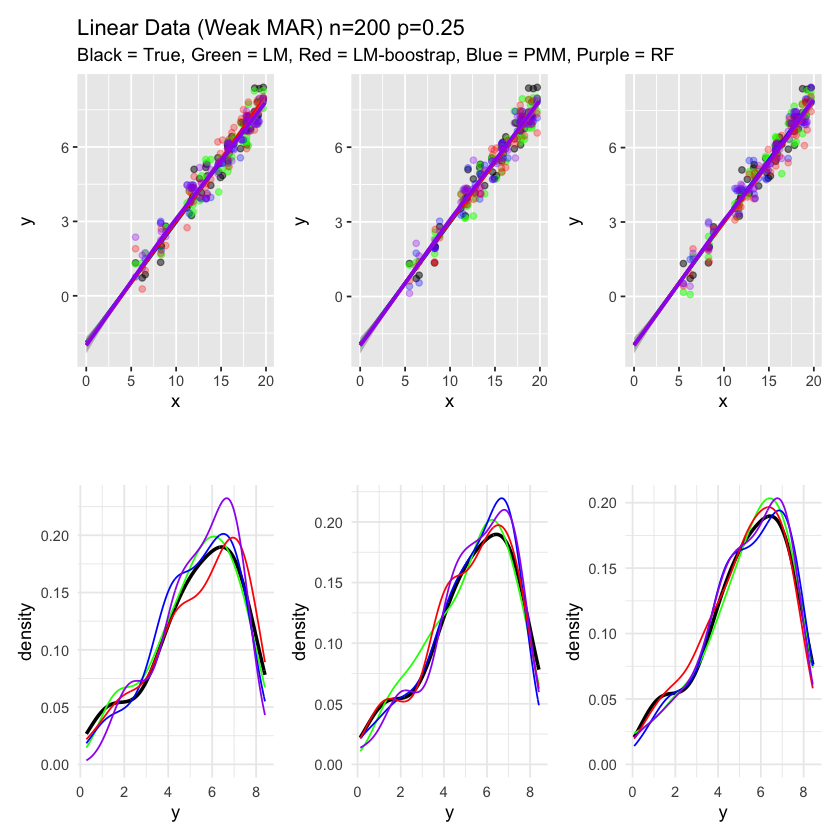
\includegraphics[width=\linewidth]{Report/Figure/linear_wmar.jpg}
    \captionof{figure}{$y$ follows a linear function of $x$, and missingness in $y$ is weakly dependent on $x$. The top row displays scatter plots comparing the imputed values (colored) to the true values (black) across three separately imputed datasets (one per column). The bottom row shows the corresponding density plots comparing the distribution of imputed values to the true distribution. All methods perform similarly due to the simplicity of the data-generating process, but nonparametric methods exhibit slightly more spread in the plots.}
    \label{fig:linear_wmar}
\end{minipage}
\hspace{1.5em}
\begin{minipage}[b]{0.48\linewidth}
    \centering
    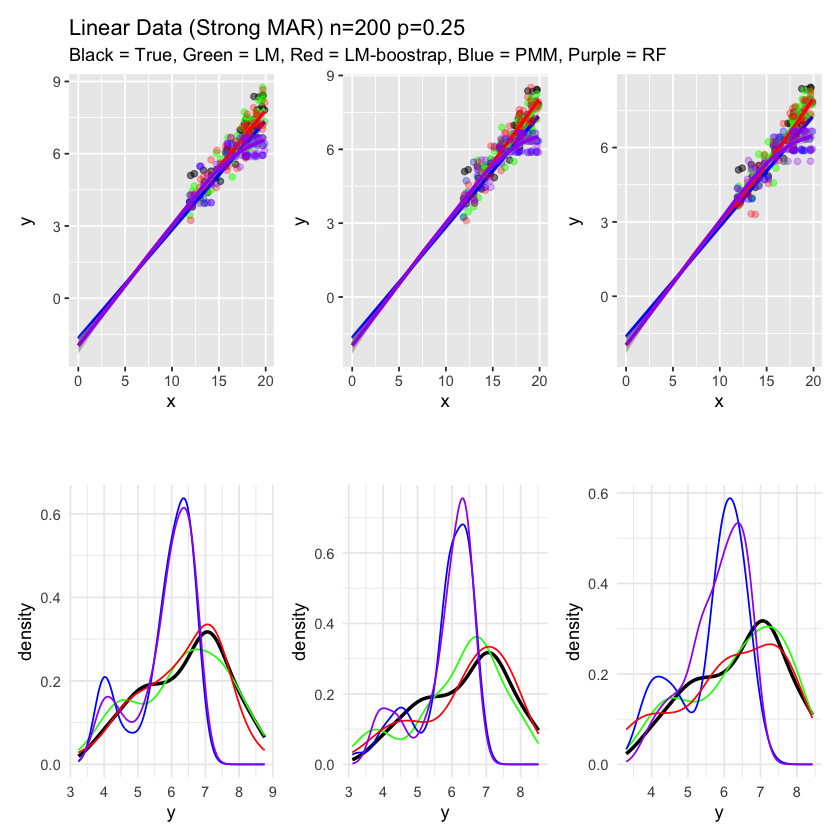
\includegraphics[width=\linewidth]{Report/Figure/linear_mar.jpg}
    \captionof{figure}{$y$ follows a linear function of $x$, and missingness in $y$ is strongly dependent on $x$. The top row displays scatter plots comparing the imputed values (colored) to the true values (black) across three separately imputed datasets (one per column). The bottom row shows the corresponding density plots comparing the distribution of imputed values to the true distribution. Parametric methods align closely with the DGP, while nonparametric methods struggle more—particularly in sparsely observed regions.}
    \label{fig:linear_mar}
\end{minipage}

\noindent
\begin{minipage}[b]{0.5\linewidth}
    \centering
    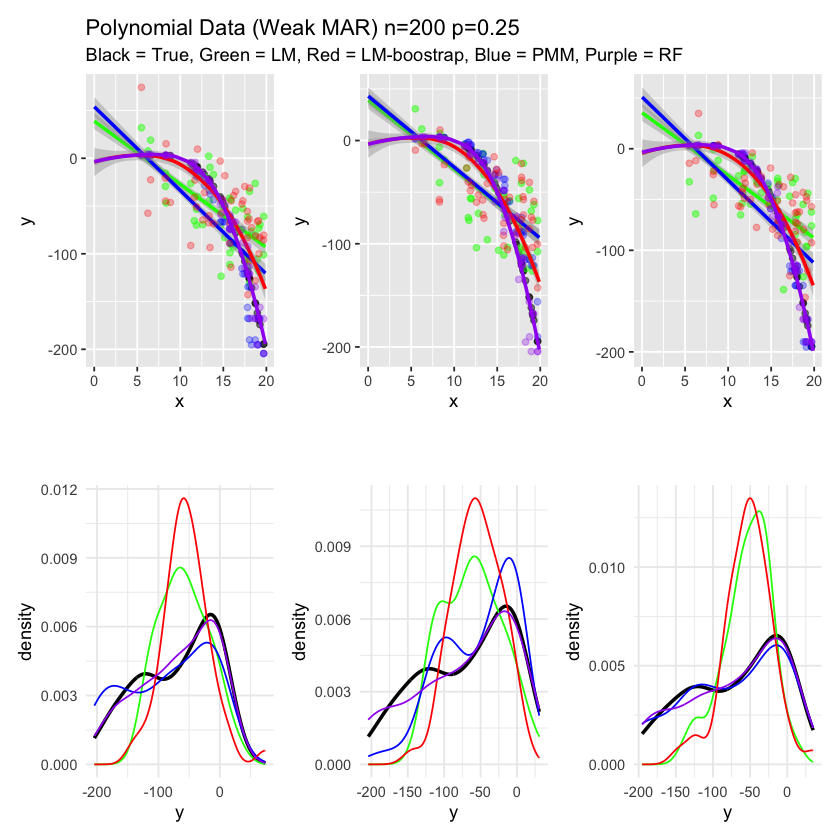
\includegraphics[width=\linewidth]{Report/Figure/poly_wmar.jpg}
    \captionof{figure}{$y$ follows a nonlinear (polynomial) function of $x$, and missingness in $y$ is weakly dependent on $x$. The top row displays scatter plots comparing the imputed values (colored) to the true values (black) across three separately imputed datasets (one per column). The bottom row shows the corresponding density plots comparing the distribution of imputed values to the true distribution. Nonparametric methods—especially RF—closely follow the nonlinear shape, while parametric methods (e.g., LM, LM-bootstrap) tend to underfit.}
    \label{fig:poly_wmar}
\end{minipage}
\hspace{1.5em}
\begin{minipage}[b]{0.5\linewidth}
    \centering
    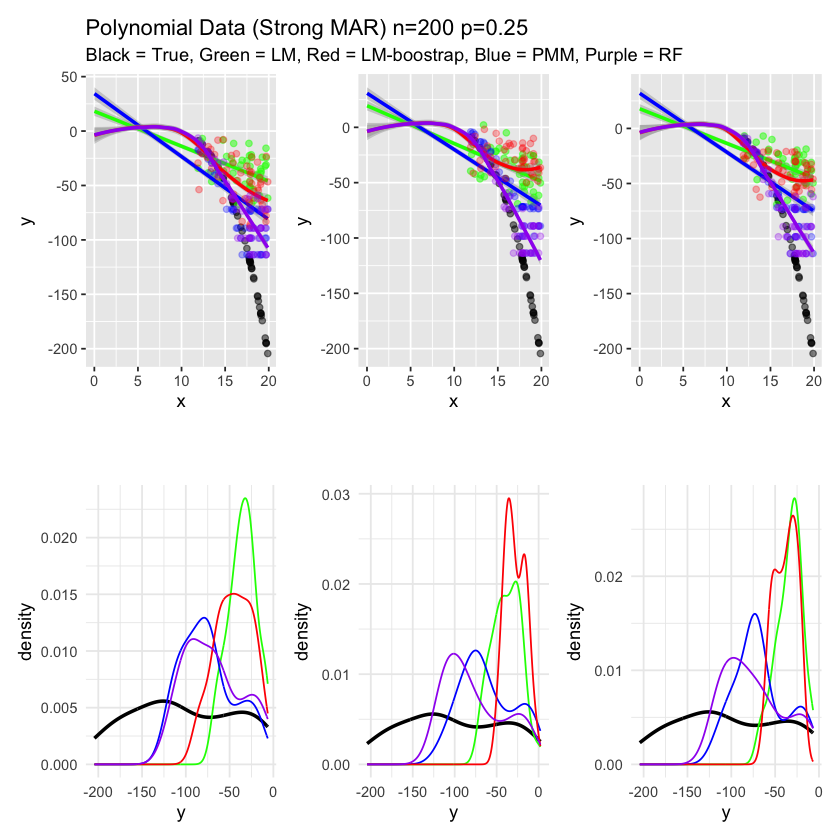
\includegraphics[width=\linewidth]{Report/Figure/poly_mar.jpg}
    \captionof{figure}{$y$ follows a nonlinear (polynomial) function of $x$, and missingness in $y$ is strongly dependent on $x$. The top row displays scatter plots comparing the imputed values (colored) to the true values (black) across three separately imputed datasets (one per column). The bottom row shows the corresponding density plots comparing the distribution of imputed values to the true distribution. All methods struggle, with parametric methods showing visibly biased imputations and nonparametric methods providing more flexible fits.}
    \label{fig:poly_mar}
\end{minipage}



\begin{table}[H]
\centering
\caption{Imputation performance for linear DGP under weak and strong MAR mechanisms. Each column corresponds to a different imputation method. Metrics include point estimation error, variance decomposition, and mean estimation error.}
\label{tab:linear}
\scalebox{0.7}{
\begin{tabular}{lrrrrrrrr}
\toprule
 & \multicolumn{4}{c}{\textbf{Weak MAR}} & \multicolumn{4}{c}{\textbf{Strong MAR}} \\
\cmidrule(lr){2-5} \cmidrule(lr){6-9}
 & \textbf{lm} & \textbf{pmm} & \textbf{boot} & \textbf{rf}
 & \textbf{lm} & \textbf{pmm} & \textbf{boot} & \textbf{rf} \\
\midrule
\textbf{RMSE}        & 0.446 & 0.524 & 0.510 & 0.600 & 0.504 & 0.984 & 0.456 & 0.955 \\
\textbf{MAE}         & 0.369 & 0.417 & 0.394 & 0.457 & 0.386 & 0.776 & 0.341 & 0.746 \\
\textbf{Wasserstein} & 0.165 & 0.244 & 0.212 & 0.240 & 0.200 & 0.678 & 0.198 & 0.647 \\
\textbf{Ubar}        & 7.492 & 7.447 & 7.405 & 7.471 & 7.383 & 6.422 & 7.381 & 6.463 \\
\textbf{Bm}          & 0.0008 & 0.0002 & 0.0010 & 0.0001 & 0.0014 & 0.0002 & 0.0008 & 0.0001 \\
\textbf{Tm}          & 7.493 & 7.448 & 7.406 & 7.471 & 7.384 & 6.422 & 7.382 & 6.464 \\
\textbf{Est\_RMSE}   & 0.036 & 0.017 & 0.041 & 0.010 & 0.054 & 0.163 & 0.050 & 0.153 \\
\textbf{Est\_MAE}    & 0.026 & 0.017 & 0.037 & 0.009 & 0.042 & 0.163 & 0.043 & 0.153 \\
\bottomrule
\end{tabular}
}
\end{table}

\begin{table}[H]
\centering
\caption{Imputation performance for polynomial DGP under weak and strong MAR mechanisms. Each column corresponds to a different imputation method. Metrics include point estimation error, variance decomposition, and mean estimation error.}
\label{tab:poly}
\scalebox{0.7}{
\begin{tabular}{lrrrrrrrr}
\toprule
 & \multicolumn{4}{c}{\textbf{Weak MAR}} & \multicolumn{4}{c}{\textbf{Strong MAR}} \\
\cmidrule(lr){2-5} \cmidrule(lr){6-9}
 & \textbf{lm} & \textbf{pmm} & \textbf{boot} & \textbf{rf}
 & \textbf{lm} & \textbf{pmm} & \textbf{boot} & \textbf{rf} \\
\midrule
\textbf{RMSE}        & 45.090 & 6.454 & 41.811 & 8.945 & 82.452 & 50.550 & 82.437 & 48.237 \\
\textbf{MAE}         & 35.287 & 4.104 & 33.803 & 5.450 & 67.349 & 35.531 & 66.587 & 32.011 \\
\textbf{Wasserstein} & 32.291 & 3.127 & 30.929 & 3.582 & 65.439 & 35.497 & 65.564 & 31.485 \\
\textbf{Ubar}        & 2090.667 & 2787.071 & 2082.552 & 2957.576 & 562.777 & 1215.113 & 562.445 & 1348.888 \\
\textbf{Bm}          & 2.758 & 10.518 & 3.084 & 0.108 & 1.230 & 1.666 & 2.433 & 0.831 \\
\textbf{Tm}          & 2093.977 & 2799.692 & 2086.253 & 2957.706 & 564.252 & 1217.112 & 565.365 & 1349.884 \\
\textbf{Est\_RMSE}   & 2.736 & 2.972 & 3.353 & 0.331 & 15.952 & 8.896 & 16.065 & 7.760 \\
\textbf{Est\_MAE}    & 2.489 & 2.606 & 3.018 & 0.230 & 15.921 & 8.821 & 16.005 & 7.717 \\
\bottomrule
\end{tabular}
}
\end{table}

In the linear DGP case, the parametric imputation methods (LM, LM with Bootstrap) align well in the density plot with the true DGP in Figures \ref{fig:linear_wmar} - \ref{fig:linear_mar}, as they directly model linear relationships. The advantage of parametric methods is more obvious when missing mechanism is strongly dependent on $x$. Nonparametric methods (PMM and RF) achieve larger RMSE, MAE and Wasserstein Distance in the point-estimate of the missing data, and also larger RMSE and MAE in the mean estimate after imputation as shown in Table \ref{tab:linear}.

In the polynomial case, parametric methods struggle, as the true relationship deviates substantially from a linear form in Figures \ref{fig:poly_wmar} - \ref{fig:poly_mar}. Nonparametric methods capture more of the underlying curvature with lower error measure in the point-estimate (RMSE, MAE and Wassersteinin Distance) and mean estimate after imputation than the parametric linear models as shown in Table \ref{tab:poly}. 

The variance components further illustrate how different imputation methods propagate uncertainty. In the linear DGP scenario, the total variance is relatively similar across all methods. However, in the polynomial DGP case—where the data exhibits more pronounced curvature and variability—parametric methods yield \textbf{substantially higher total variance}, reflecting both their greater flexibility and the \textbf{increased variability in their predictions}. The variance components further illustrate how different imputation methods propagate uncertainty. In both linear and polynomial DGPs, we observe that total variance tends to be lower under strong MAR compared to weak MAR. This trend may be due to the fact that strong MAR induces missingness in more structured regions of the covariate space, which can reduce the variability of plausible imputations. As a result, all methods exhibit lower total variance, potentially underestimating uncertainty. This highlights that the nature of missingness also plays a central role in the variance behavior of imputations.

\subsection{Simulation Results}
We now look at simulation results across different levels of missing proportion from $5\%$ to $60\%$.

In the \textbf{linear DGP} setting, under \textbf{weak MAR} where missingness is only mildly related to the predictor $x$, all methods perform comparably and exhibit \textbf{stable behavior} across increasing missing proportions up to $p=0.6$ for error metrics (RMSE, MAE, Wasserstein Distance) in missing data point-estimates. Variance components ($\bar{U}, B_M, T_M$) show gradual, non-rapid growth growth in trend. The mean estimator metrics (Estimate RMSE and MAE) show modest growth in trend as well but remain below $0.04$. These results suggest that when the missingness mechanism is nearly ignorable and the relationship between the missing variable and covariate is simple, both parametric and nonparametric imputation methods can perform reliably and consistently across a range of missingness levels (Figures \ref{fig:result_linear_wmar} and  \ref{fig:mean_linear_wmar}).

In contrast, under \textbf{strong MAR} where the probability of missingness strongly depends on $x$, model performance diverges significantly. Nonparametric methods (PMM and RF) suffer from increases in point estimate RMSE, MAE, and Wasserstein Distance as missing proportion increases, while parametric methods remain remarkably stable. This behavior suggests that parametric models are more robust to non-ignorable missingness, provided their \textbf{modeling assumptions hold}. In contrast, nonparametric methods are \textbf{more sensitive to informative missingness}. We observe a similar trend in the error measures for the mean estimates after imputation. Variance metrics $\bar{U}$ and $T_M$ for nonparametric methods decline with increasing missingness. This could reflect \textbf{underestimated uncertainty}, as these nonparametric methods rely on observed data instead of assumptions of the underlying model. Additionally, with fewer observed points, imputed values can become overly concentrated, reducing apparent variance despite decreasing accuracy. However, \textbf{further investigation is needed} to understand the exact causes and implications of the results  (Figures \ref{fig:result_linear_mar} and  \ref{fig:mean_linear_mar}). \\

\begin{figure}[ht]
    \centering
    \begin{minipage}[b]{0.48\linewidth}
        \centering
        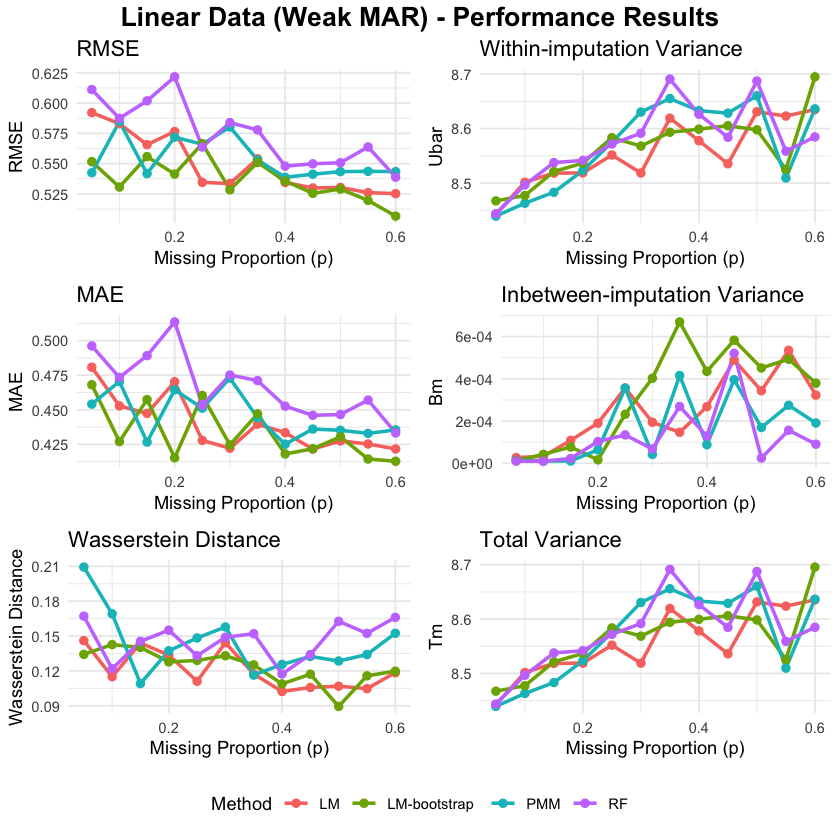
\includegraphics[width=\linewidth]{Report/Figure/result_linear_wmar.jpg}
        \caption{Plot for the changes in point-estimate error (RMSE, MAE, Wasserstein), and variance components ($\bar{U}$, $B_M$, $T_M$), across increasing missingness levels under the \textbf{weak MAR} mechanism with \textbf{linear DGP} ($p$ representing the missing data proportion).}
        \label{fig:result_linear_wmar}
    \end{minipage}
    \hfill
    \begin{minipage}[b]{0.48\linewidth}
        \centering
        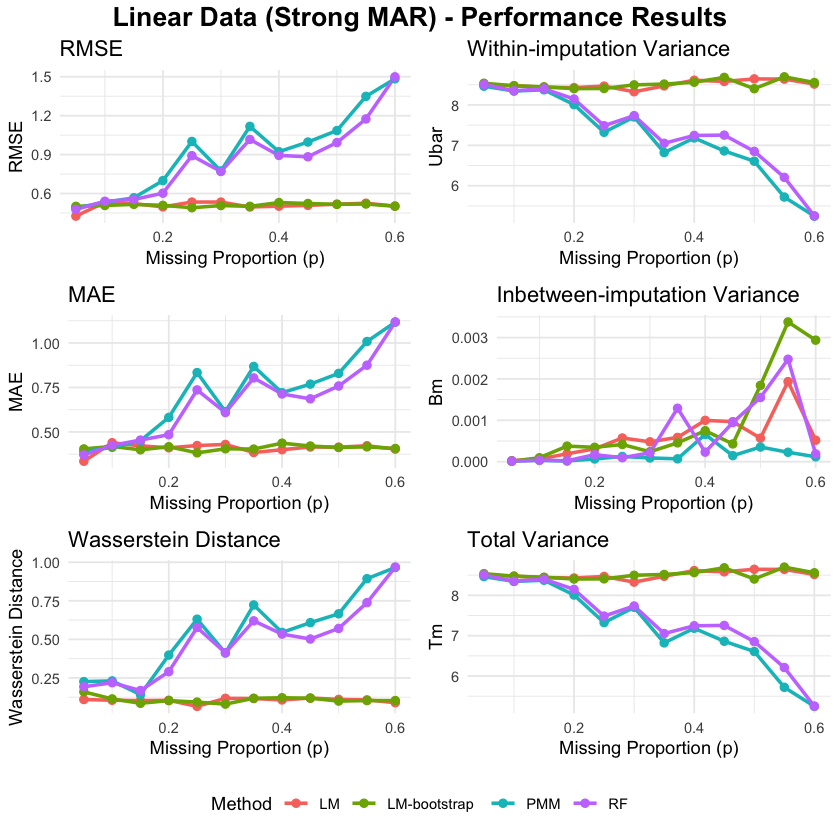
\includegraphics[width=\linewidth]{Report/Figure/result_linear_mar.jpg}
        \caption{Plot for the changes in point-estimate error (RMSE, MAE, Wasserstein), and variance components ($\bar{U}$, $B_M$, $T_M$), across increasing missingness levels under the \textbf{strong MAR} mechanism with \textbf{linear DGP} ($p$ represents the missing data proportion).}
        \label{fig:result_linear_mar}
    \end{minipage}
\end{figure}

\begin{figure}[ht]
    \centering
    \begin{minipage}[b]{0.48\linewidth}
        \centering
        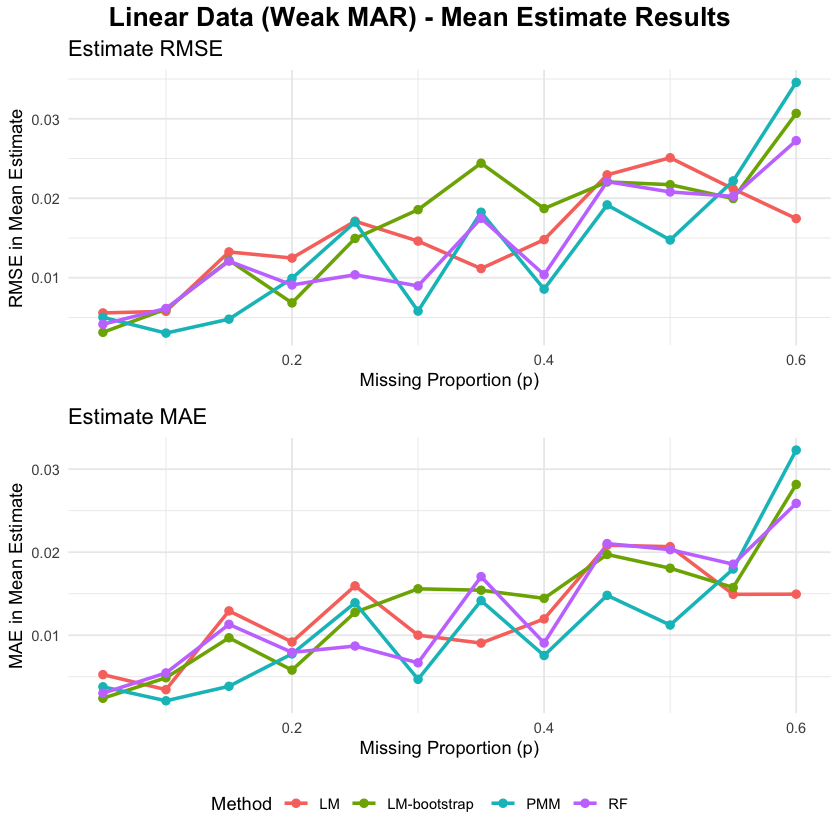
\includegraphics[width=\linewidth]{Report/Figure/mean_linear_wmar.jpg}
        \caption{Plot for the changes in mean estimate error (RMSE, MAE) across increasing missingness levels under the \textbf{weak MAR} mechanism with \textbf{linear DGP} ($p$ represents the missing data proportion).}
        \label{fig:mean_linear_wmar}
    \end{minipage}
    \hfill
    \begin{minipage}[b]{0.48\linewidth}
        \centering
        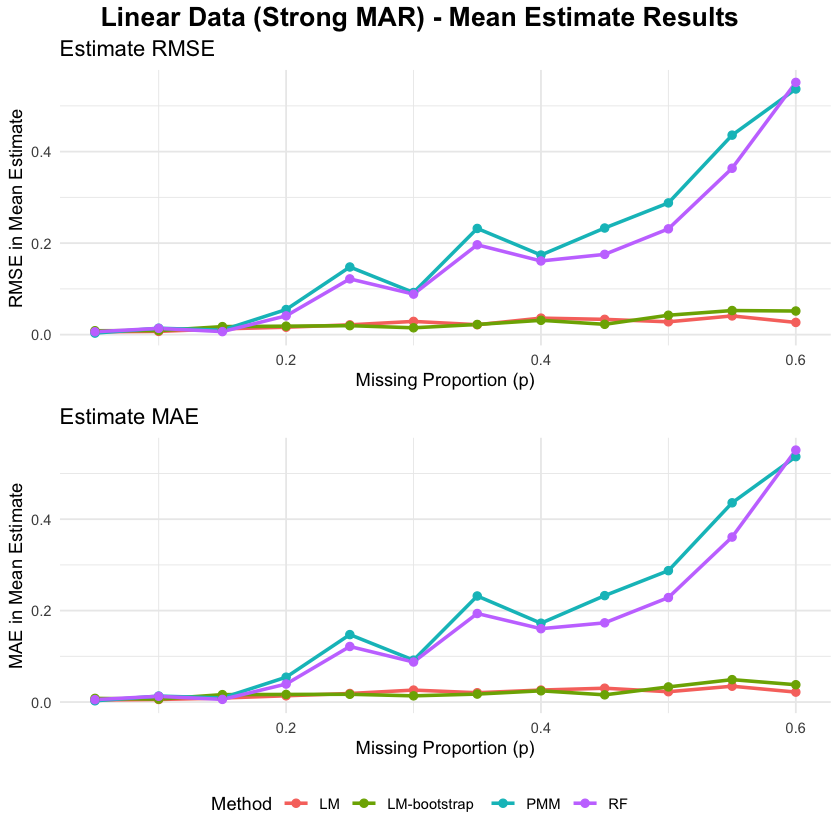
\includegraphics[width=\linewidth]{Report/Figure/mean_linear_mar.jpg}
        \caption{Plot for the changes in mean estimate error (RMSE, MAE) across increasing missingness levels under the \textbf{strong MAR} mechanism with \textbf{linear DGP} ($p$ represents the missing data proportion).}
        \label{fig:mean_linear_mar}
    \end{minipage}
\end{figure}

In the \textbf{polynomial DGP} setting, under the \textbf{weak MAR} scenario, parametric methods (LM and LM-bootstrap) consistently yield high RMSE and MAE, indicating systematic bias due to their disadvantage in capturing the nonlinear structure of the data. In contrast, nonparametric methods—particularly RF—demonstrate substantially lower and more stable error across missingness levels, especially in mean estimation. The total variances for nonparametric methods remain relatively stable but are much higher than that of parametric methods, suggesting better adaptation to the data-generating process (DGP) but also greater uncertainty in imputation. Meanwhile, the decreasing variance observed in parametric methods may indicate overconfidence despite poor fit (Figures \ref{fig:result_poly_wmar} and  \ref{fig:mean_poly_wmar}).

In the \textbf{strong MAR} setting, trends become more complex. While nonparametric methods generally maintain lower point estimation error and mean estimation error than parametric methods, parametric methods show obvious \textbf{decreasing trends} as $p$ increases. One possible explanation is that the missingness under strong MAR is concentrated in regions where the parametric model already performs poorly—such as highly nonlinear areas—so removing more of that challenging data effectively simplifies the task for the misspecified model. This can artificially improve performance metrics despite the underlying misfit. In this case, the apparent improvement reflects \textbf{selective bias due to missing data} rather than genuine model robustness. However, it \textbf{requires further investigation} to confirm. Nonparametric methods maintain higher total variance in general, which aligns with their greater modeling flexibility. However, what is less expected is the \textbf{overall decrease in variance} across all methods as missingness increases. This trend may again reflect reduced variability in imputed values due to less observed data as in the linear DGP cases, leading to fewer distinct imputation possibilities. It again highlights a subtle but important interaction between missingness structure and model behavior that deserves further exploration (Figures \ref{fig:result_poly_mar} and  \ref{fig:mean_poly_mar}).





\begin{figure}[ht]
    \centering
    \begin{minipage}[b]{0.48\linewidth}
        \centering
        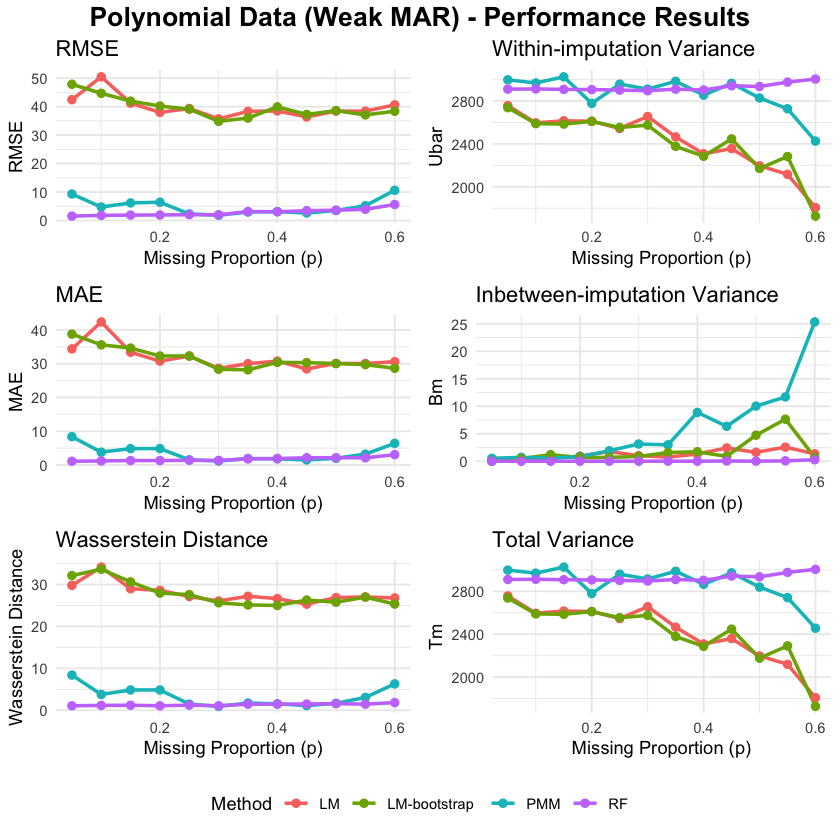
\includegraphics[width=\linewidth]{Report/Figure/result_poly_wmar.jpg}
        \caption{Plot for the changes in point-estimate error (RMSE, MAE, Wasserstein), and variance components ($\bar{U}$, $B_M$, $T_M$), across increasing missingness levels under the \textbf{weak MAR} mechanism with \textbf{polynomial DGP}, with $p$ representing the missing data proportion.}
        \label{fig:result_poly_wmar}
    \end{minipage}
    \hfill
    \begin{minipage}[b]{0.48\linewidth}
        \centering
        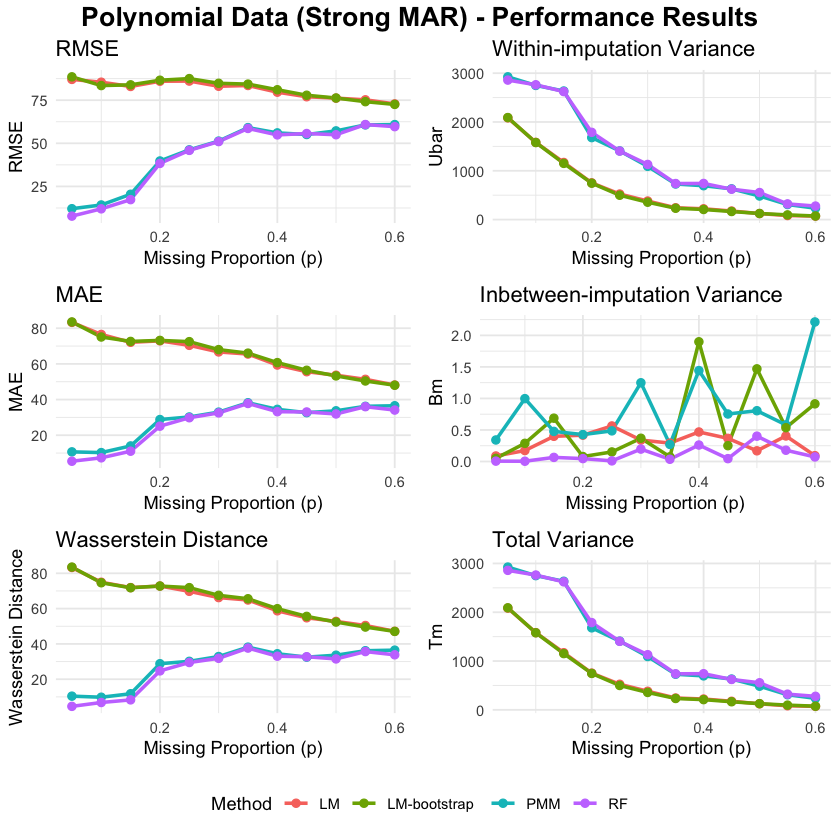
\includegraphics[width=\linewidth]{Report/Figure/result_poly_mar.jpg}
        \caption{Plot for the changes in point-estimate error (RMSE, MAE, Wasserstein), and variance components ($\bar{U}$, $B_M$, $T_M$), across increasing missingness levels under the \textbf{strong MAR} mechanism with \textbf{polynomial DGP}, with $p$ representing the missing data proportion.}
        \label{fig:result_poly_mar}
    \end{minipage}
\end{figure}

\begin{figure}[ht]
    \centering
    \begin{minipage}[b]{0.48\linewidth}
        \centering
        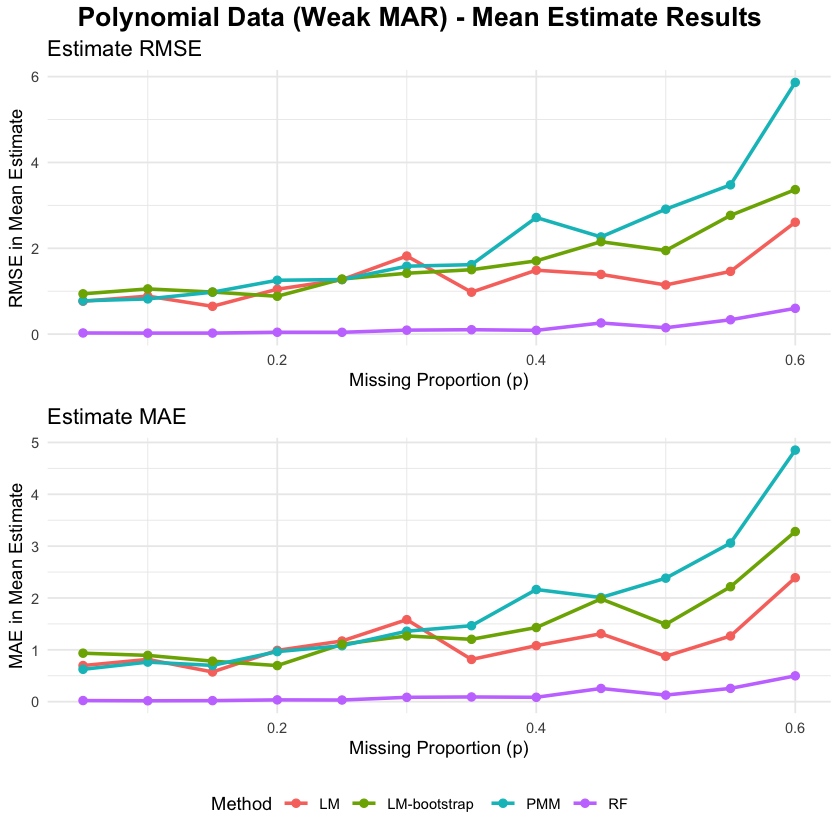
\includegraphics[width=\linewidth]{Report/Figure/mean_poly_wmar.jpg}
        \caption{Plot for the changes in mean estimate error (RMSE, MAE) across increasing missingness levels under the \textbf{weak MAR} mechanism with \textbf{polynomial DGP} ($p$ represents the missing data proportion).}
        \label{fig:mean_poly_wmar}
    \end{minipage}
    \hfill
    \begin{minipage}[b]{0.48\linewidth}
        \centering
        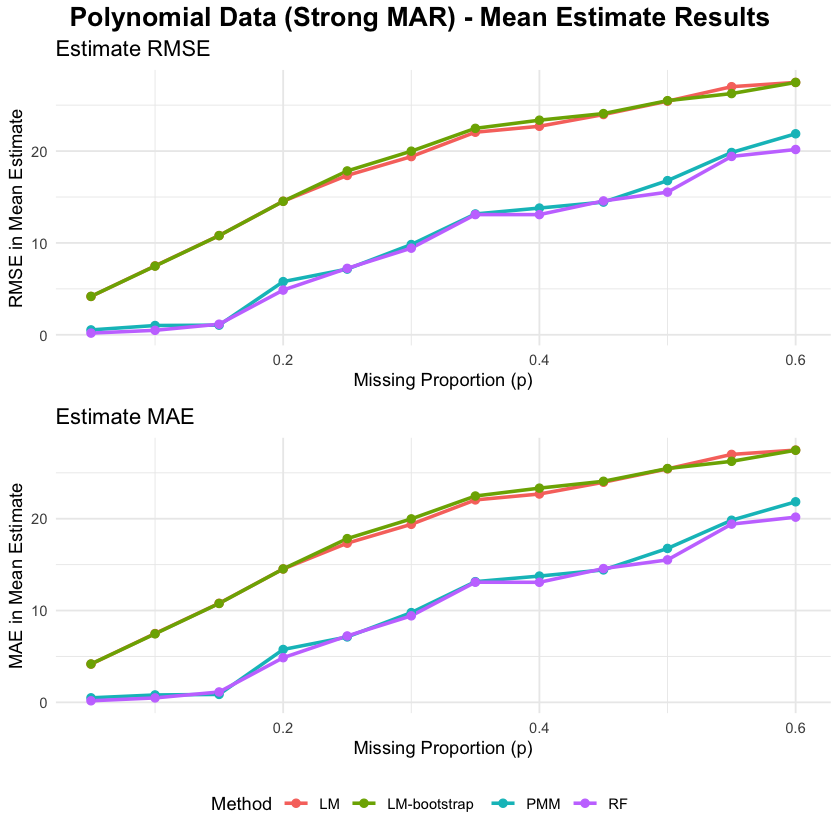
\includegraphics[width=\linewidth]{Report/Figure/mean_poly_mar.jpg}
        \caption{Plot for the changes in mean estimate error (RMSE, MAE) across increasing missingness levels under the \textbf{strong MAR} mechanism with \textbf{polynomial DGP} ($p$ represents the missing data proportion).}
        \label{fig:mean_poly_mar}
    \end{minipage}
\end{figure}
\subsection{Conclusion.}
All the simulations are done in \textit{R} and the code can be found on GitHub: \url {https://github.com/zhoumo2716/QP5-for-submission}. In summary, these results reveal a nuanced interaction between imputation method, data structure, and missingness mechanism. Parametric models tend to perform well when the data-generating process (DGP) aligns with their assumptions—even under strong MAR—but break down when applied to nonlinear structures. In contrast, nonparametric methods demonstrate greater robustness to model misspecification and perform better in more complex DGPs. However, they often yield higher variance and may degrade more sharply under informative missingness. The comparison between weak and strong MAR scenarios further underscores that the \textbf{nature of missingness—not just its proportion—plays a crucial role} in shaping both imputation accuracy and uncertainty quantification. These findings highlight the importance of selecting imputation strategies that are well-suited to the underlying data structure and realistic assumptions about missingness, balancing the trade-offs between parametric simplicity and nonparametric flexibility. 

\clearpage
\printbibliography
\end{document}
